%%% template.tex
%%%
%%% This LaTeX source document can be used as the basis for your technical
%%% paper or abstract.

%%% The parameter to the ``documentclass'' command is very important.
%%% - use ``review'' for content submitted for review.
%%% - use ``preprint'' for accepted content you are making available.
%%% - use ``tog'' for technical papers accepted to the TOG journal and
%%%   for presentation at the SIGGRAPH or SIGGRAPH Asia conference.
%%% - use ``conference'' for final content accepted to a sponsored event
%%%   (hint: If you don't know, you should use ``conference.'')

\documentclass[tog]{acmsiggraph}

\usepackage{array}
\usepackage{amssymb}
\usepackage[ngerman]{babel}
\usepackage[utf8]{inputenc}
\usepackage{tikz}
\usetikzlibrary{arrows,chains,matrix,positioning,scopes}

%%% Make the ``BibTeX'' word pretty...

\def\BibTeX{{\rm B\kern-.05em{\sc i\kern-.025em b}\kern-.08em
    T\kern-.1667em\lower.7ex\hbox{E}\kern-.125emX}}

%%% Used by the ``review'' variation; the online ID will be printed on 
%%% every page of the content.

\TOGonlineid{45678}

%%% Used by the ``preprint'' variation.

\TOGvolume{0}
\TOGnumber{0}

\title{Ausarbeitung zum Thema der ganzzahligen linearen Programmierung (ILP)}

\author{Patric Vormstein\\Seminar Lineare und ganzzahlige lineare Programmierung, SoSe 2015\\Leitung: Prof. Dr. Ernst Althaus}
\pdfauthor{Stephen N. Spencer}

\keywords{radiosity, global illumination, constant time}

\begin{document}

%%% This is the ``teaser'' command, which puts an figure, centered, below 
%%% the title and author information, and above the body of the content.

 \teaser{
   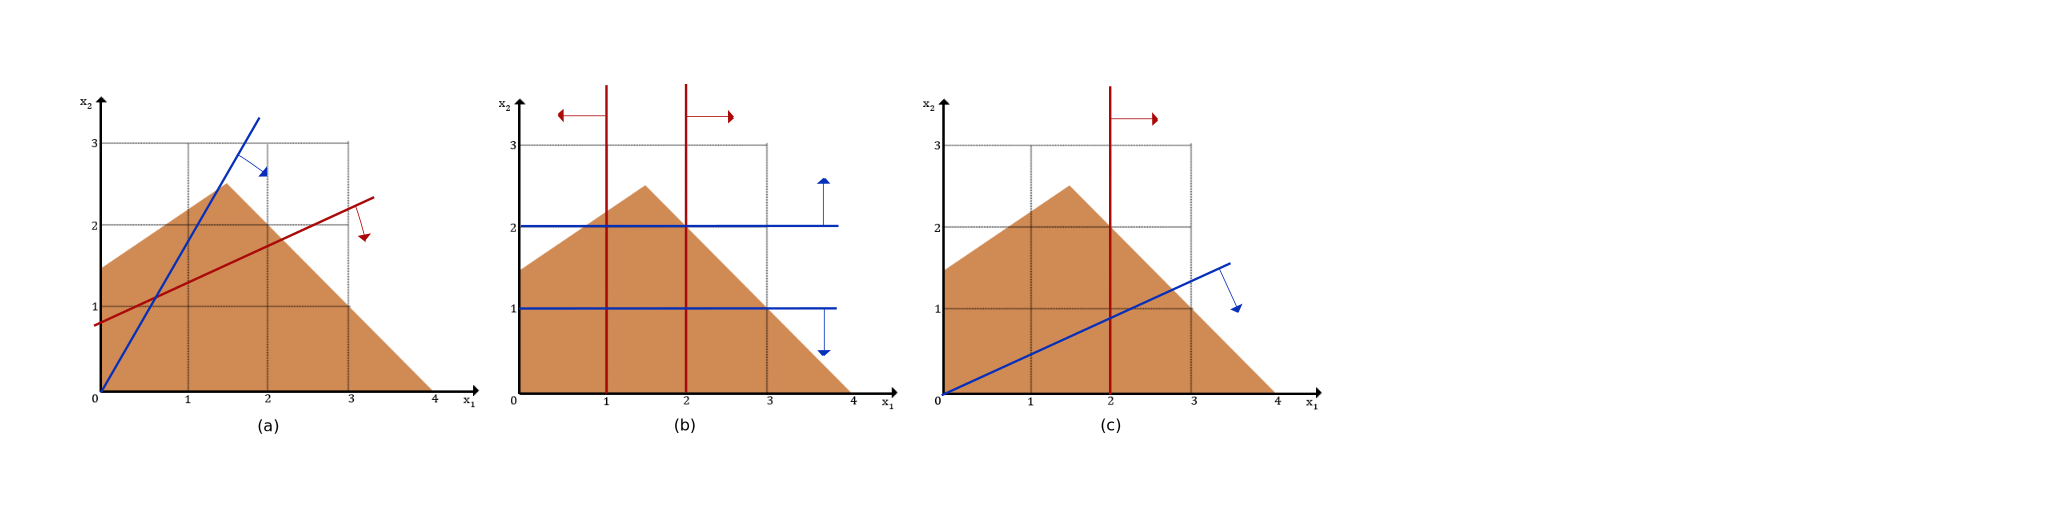
\includegraphics[height=1.8in]{images/teaser}
   \caption{Beispielhafte Darstellungen der Algorithmen die in dieser Ausarbeitung vorgestellt werden. (a) zeigt das Gomory-Schnittebenenverfahren. (b) stellt den Branch-and-Bound-Algorithmus dar. (c) ist eine Dartstellung des Branch-and-Cut-Verfahrens.}
 }

\maketitle

\begin{abstract}

Diese Ausarbeitung setzt sich mit der ganzzahligen linearen Programmierung (oder ILP für \textit{integer linear programming}) auseinander und stellt drei exakte Algorithmen zum Lösen von ganzzahligen linearen Problemen vor.\\
Dabei handelt es sich um das Gomory-Schnittebenenverfahren, dem Branch-and-Bound-Algorithmus und ein Verfahren, dass die Vorteile beider Algorithmen nutzt, und zwar das Branch-and-Cut.\\
Ein besonderes Augenmerk soll hier auf die praktische Anwendung der Algorithmen gelegt werden.\\
Für diese Ausarbeitung werden nicht-ganzzahlige lineare Probleme (LP), feasible bzw. zulässige Lösungen und der Simplex-Algorithmus (inkl. optimalem Tableau) als bekannt vorausgesetzt.\\
Desweiteren liegt dieser Ausarbeitung das Buch \textit{Introduction to linear Optimization} (Kapitel 11, S. 479 - 490) von \textsc{Dimitris Bertsimas} und \textsc{John N. Tsitsiklis} zugrunde.
\end{abstract}

%% Required for all content. 

%\copyrightspace

\section{Grundlagen}

Bevor auf die Algorithmen eingegangen wird müssen vorher noch die Grundlagen zu diesem Thema erläutert werden.\\
Als Anfangspunkt betrachten wir im Folgenden (\ref{Eq:LP}) eine bereits bekannte Form für ein generisches lineares Problem:

\large
\begin{align}
\label{Eq:LP}
minimize \;\; c'x & \nonumber \\
subject \;\; to \;\; Ax &= b \nonumber \\
x &\geq 0
\end{align}
\normalsize

Durch eine Modifikation der Lösungsvoraussetzung des Problems können wir das Problem in ein ganzzahliges Problem ändern. Wir beschränken die Lösungen auf Ganzzahligkeit. Dadurch erhalten wir folgende Form (\ref{Eq:ILP}) und somit eine ILP:

\large
\begin{align}
\label{Eq:ILP}
minimize \;\; c'x & \nonumber \\
subject \;\; to \;\; Ax &= b \nonumber \\
x &\geq 0 \nonumber \\
x \;\; &integer
\end{align}
\normalsize

Der Grund weshalb wir zuerst die nicht-ganzzahlige LP betrachtet haben liegt darin, dass sich jede ILP durch Wegnahme der Ganzzahligkeitsbeschränkung in eine sogenannte \textit{LP-Relaxierung} umwandeln lässt. Somit ist die LP aus der Gleichung \ref{Eq:LP} die LP-Relaxierung zur ILP aus Gleichung \ref{Eq:ILP}.

Die LP-Relaxierung dient dazu die Lösungssuche zu einer bestimmten ILP zu erleichtern, da es sich bei der Lösung von ILPs um ein NP-schweres Problem handelt. Daraus folgt, dass keine effizienten Algorithmen existieren.\\
Die Algorithmen denen man sich zur Lösung bedient lassen sich in drei Kategorien einteilen:

\begin{enumerate}
\item Exakte Algorithmen
\begin{itemize}
\item Berechnen eine optimale Lösung
\item Haben eine exponentielle Laufzeit
\end{itemize}
\item Approximierende Algorithmen
\begin{itemize}
\item Berechnen lediglich suboptimale Lösung
\item Haben dafür eine polynomielle Laufzeit
\end{itemize}
\item Heuristische Algorithmen
\begin{itemize}
\item Berechnen ohne Garantie eine suboptimale Lösung
\item Haben im besten Fall polynomielle Laufzeit, kann aber auch exponentiell sein
\item Meistens berechnen sie brauchbare Ergebnisse
\end{itemize}
\end{enumerate}

Die Algorithmen die wir in den folgenden Abschnitten beleuchten werden stammen aus der ersten Kategorie. Es handeln sich um exakte Algorithmen. 

\section{Schnittebenenverfahren}

\subsection*{Grundidee}

Betrachten wir nun erneut die ILP aus Gleichung \ref{Eq:ILP} und versuchen sie nun zu lösen.\\
Dabei verwenden wir folgende Lösungsschritte:
\begin{enumerate}
\item Bilde die LP-Relaxierung der ILP. Diese ist uns bereits aus Gleichung \ref{Eq:LP} bekannt.\\ Nun sei $x^{*}$ die optimale Lösung zur LP-Relaxierung.
\item Falls $x^{*}$ ganzzahlig ist, dann ist $x^{*}$ ebenfalls die optimale Lösung zur ILP und der Algorithmus hält an.
\item Falls $x^{*}$ nicht ganzzahlig ist, dann fügen wir eine weitere Bedingung hinzu, die der optimalen Lösung der LP-Relaxierung widerspricht, aber nicht der optimalen Lösung der ILP.\\
Dazu betrachten wir folgendes Beispiel mit $x^{*}$ als optimale Lösung zur LP-Relaxierung:\\

\subsubsection*{Beispiel}
Sei $x^{*}_{i}$ ein Bruch mit:
\large
\begin{equation}
\frac{p}{q} \in \mathbb{Q},\;\; p < q \nonumber
\end{equation}
\normalsize

Damit ist $x^{*}$ keine optimale Lösung der ILP.\\
Durch Hinzunahme der Bedingung $x^{*}_{i} \ge 1$ zur LP-Relaxierung können wir die Lösungssuche verfeinern.\\
$x^{*}$ ist somit keine zulässige Lösung der LP-Relaxierung.

\item Mit dieser neuen Bedingung berechnen wir erneut eine Lösung für die LP-Relaxierung und beginnen wieder bei Schritt 1.

\end{enumerate}

Das Hinzufügen neuer Bedingungen kann man auch als \textit{Abschneiden unbrauchbarer Lösungen} bezeichnen. Dies führt uns zu sogenannten \textit{Schnittebenen}.\\
Durch ständiges Abschneiden unbrauchbarer Lösung erlangt man mit der Zeit eine ganzzahlige Lösung in der LP-Relaxierung.\\
Die Problematik besteht hingegen darin geeignete Schnittebenen zu bestimmen.\\
Im Jahre 1958 hat Ralph Gomory ein entsprechend brauchbares Verfahren zum Bestimmen solcher Schnittebenen entwickelt welches im Folgenden vorgestellt wird.

\subsection*{Gomory-Schnittebenenverfahren}

Das Verfahren von Ralph Gomory baut auf dem als hier bekannt vorausgesetztem Simplex-Algorithmus auf.\\
Führen wir den Simplex-Algorithmus auf einer LP-Relaxierung aus, so erhalten wir eine Lösung folgender Form:

\large
\begin{align}
\label{Eq:Simplex}
B^{-1} Ax = B^{-1}b
\end{align}
\normalsize

Das dazugehörige optimale Tableau sieht beispielsweise wie folgt aus:

\begin{table}[ht]
\centering
\caption{Optimales Tableau einer bestimmten LP-Relaxierung}
\label{Tb:Optimales Tableau}
\begin{tabular}{lllll}
& $x_1$ & $x_2$  & $x_3$ & $x_4$ \\
\hline
\multicolumn{1}{|l|}{\large$a_{00}$} & \large$a_{01}$  & \large$a_{02}$ & \large$a_{03}$ & \multicolumn{1}{l|}{\large$a_{04}$} \\ \hline
\multicolumn{1}{|l|}{\large$a_{10}$} & \large$a_{11}$ & \large$a_{12}$ & \large$a_{13}$ & \multicolumn{1}{l|}{\large$a_{14}$} \\
\multicolumn{1}{|l|}{\large$a_{20}$} & \large$a_{21}$ & \large$a_{22}$ & \large$a_{23}$ & \multicolumn{1}{l|}{\large$a_{24}$} \\ \hline               
\large$\underbrace{}_{B^{-1}b}$ &   &   & \multicolumn{2}{l}{\large$\underbrace{\;\;\;\;\;\;\;\;\;\;\;\;\;\;\;\;}_{B^{-1}A_N}$}      
\end{tabular}
\end{table}

Betrachten wir das Ergebnis des Simplex-Algorithmus genauer, so können wir es in Basis-Variablen und Nicht-Basis-Variablen aufteilen. Wir erhalten dann folgende Form:

\large
\begin{align}
\label{Eq:SimplexBasis}
x_B + B^{-1} A_N x_N = B^{-1}b
\end{align}
\normalsize

Dabei seien $x_B$ die Basis-Variablen und $x_N$ die Nicht-Basis-Variablen und $A_N$ die Submatrix mit den Koeffizienten der Nicht-Basis-Variablen.\\
Angenommen in unserem optimalem Tableau der Tabelle \ref{Tb:Optimales Tableau} seien $x_1$ und $x_2$ die Basis-Variablen, dann sind die Spalten von $x_3$ und $x_4$ die Nicht-Basis-Koeffizienten.\\
Diese können wir zusammenfassen als $\bar{a}_{ij} = (B^{-1} A_j)_i$. \\
Die Ergebnisspalte des optimalem Tableau beschreiben wir mit $\bar{a}_{i0} = (B^{-1} b)_i$.

Nun selektieren wir aus dem optimalem Tableau eine Zeile, in der $\bar{a}_{i0}$ nicht ganzzahlig ist. Diese hat dann folgende Form:

\large
\begin{align}
\label{Eq:Gomory Schritt 1}
x_i + \sum_{j \in N} \bar{a}_{ij} x_{j} = \bar{a}_{i0}
\end{align}
\normalsize

Wir können nun die Koeffizienten der Nicht-Basis-Variablen abrunden und erhalten eine Gleichung die kleiner oder gleich der Gleichung \ref{Eq:Gomory Schritt 1} ist:

\large
\begin{align}
\label{Eq:Gomory Schritt 2}
 x_i + \sum_{j \in N} \lfloor\bar{a}_{ij}\rfloor x_{j} \leq x_i + \sum_{j \in N} \bar{a}_{ij} x_{j} = \bar{a}_{i0}
\end{align}
\normalsize

Durch den Zwischenschritt ist es jetzt möglich das $\bar{a}_{i0}$ ebenfalls abzurunden ohne die (Un)Gleichung zu verletzen:

\large
\begin{align}
\label{Eq:Gomory-Bedingung}
 x_i + \sum_{j \in N} \lfloor\bar{a}_{ij}\rfloor x_{j} \leq \lfloor \bar{a}_{i0} \rfloor
\end{align}
\normalsize

Diese neue Ungleichung \ref{Eq:Gomory-Bedingung} ist unsere neue Schnittbedingung da sie alle zulässigen nicht-ganzzahligen Lösungen hinter dieser Schnittebene \textit{abschneidet}.\\
Durch Hinzufügen der neuen Bedingung zur LP-Relaxierung lässt sich nun erneut der Simplex-Algorithmus durchführen. Dies wird solange wiederholt bis eine ganzzahlige Lösung gefunden wird.

\subsection*{Beispiel des Gomory-Verfahren}

\begin{figure*}[t!]
  \centering
  \includegraphics[scale=0.40]{images/gomory-example}
  \caption{Graphische Darstellung des Gomory-Beispiels. (a) zeigt die erste optimale nicht-ganzzahlige Lösung $x^{*}$. (b) zeigt in roter Farbe den ersten Gomory-Schnitt und in blau die zweite optimale nicht-ganzzahlige Lösung $x^{**}$ der LP-Relaxierung. (c) zeigt in blau den neuen Gomory-Schnitt und die optimale ganzzahlige Lösung $x^{***}$ der ILP. }
  \label{fig:gomory-example}
\end{figure*}

Für das Beispiel betrachten wir folgende ILP:

\large
\begin{align}
\label{Eq:Gomory-Beispiel-ILP}
minimize \;\; x_1 - 2x_2 & \nonumber \\
subject \;\; to \;\; -4x_1 + 6x_2 &\leq 9 \nonumber \\
x_1 + x_2 &\leq 4 \nonumber \\
x_1, x_2 &\geq 0 \nonumber \\
x_1, x_2 \;\; &integer
\end{align}
\normalsize

In Anbetracht des Simplex-Algorithmus müssen wir die ILP nun auch in die Normalform umwandeln:

\large
\begin{align}
\label{Eq:Gomory-Beispiel-ILP-Normal}
minimize \;\; x_1 - 2x_2 & \nonumber \\
subject \;\; to \;\; -4x_1 + 6x_2 + x_3 &= 9 \nonumber \\
x_1 + x_2 + x_4 &= 4 \nonumber \\
x_1, ..., x_4 &\geq 0 \nonumber \\
x_1, ..., x_4 \;\; &integer
\end{align}
\normalsize

\subsubsection*{1. Iteration}

Nach Anwendung des Simplex-Algorithmus erhalten wir folgendes optimales Tableau:


\begin{table}[ht]
\begin{center}

\centering
\caption{Optimales Tableau zum Gomory-Beispiel in der ersten Iteration}
\label{Tb:Optimales Tableau Gomory Beispiel}
%\begin{tabular}{*5{>{\centering\arraybackslash}m{20pt}} @{}m{0pt}@{}}
\begin{tabular}{ccccc}
%\begin{tabular}{>{\centering\bfseries}m{30pt} >{\centering}m{30pt} >{\centering}m{30pt} >{\centering}m{30pt} >{\centering\arraybackslash}m{30pt}}
& $x_1$ & $x_2$  & $x_3$ & $x_4$ \\
\hline
\multicolumn{1}{|c|}{\rule{0pt}{3.5ex}\large$-\frac{7}{2}$} & \large$0$  & \large$0$ & \large$-\frac{3}{10}$ & \multicolumn{1}{c|}{\large$-\frac{1}{5}$} \\[2ex] \hline
\multicolumn{1}{|c|}{\rule{0pt}{3.5ex}\large$\frac{5}{2}$} & \large$0$ & \large$1$ & \large$\frac{1}{10}$ & \multicolumn{1}{c|}{\large$\frac{2}{5}$} \\[2ex]
\multicolumn{1}{|c|}{\rule{0pt}{3.5ex}\large$\frac{3}{2}$} & \large$1$ & \large$0$ & \large$-\frac{1}{10}$ & \multicolumn{1}{c|}{\large$-\frac{3}{5}$} \\[2ex] \hline                 
\end{tabular}
\end{center}
\end{table}

Aus der Tabelle können wir die erste optimale Lösung ablesen mit $x^* = (\frac{3}{2}, \frac{5}{2})$. In Abbildung \ref{fig:gomory-example} (a) wird dies graphisch verdeutlicht.\\
Da es sich dabei um eine nicht-ganzzahlige Lösung handelt muss nun der Gomory-Algorithmus angewendet werden. Dazu selektieren wir die erste Zeile, in der eine Basis-Variable vorkommt und $\bar{a}_{i0}$ keine Ganzzahl ist.\\
Wir selektieren also die zweite Zeile in dieser Form:

\large
\begin{align}
\label{Eq:Gomory-Beispiel It 1}
x_2 + \frac{1}{10} x_3 + \frac{2}{5} x_4 = \frac{5}{2}
\end{align}
\normalsize

Nach dem Gomory-Verfahren müssen wir nun die Koeffizienten der Nicht-Basis-Variablen abrunden um unsere Schnittebene zu erhalten:

\large
\begin{align}
\label{Eq:Gomory-Beispiel It 1 - 2}
x_2 + \lfloor \frac{1}{10}\rfloor x_3 + \lfloor\frac{2}{5}\rfloor x_4 &\leq x_2 + \frac{1}{10} x_3 + \frac{2}{5} x_4 = \frac{5}{2} \nonumber \\
x_2 &\leq \lfloor \frac{5}{2} \rfloor \nonumber \\
x_2 &\leq 2
\end{align}
\normalsize

Unsere ILP in Normalform sieht mit der neuen Bedingung dann wie folgt aus:

\large
\begin{align}
\label{Eq:Gomory-Beispiel-ILP-Normal-It2}
minimize \;\; x_1 - 2x_2 & \nonumber \\
subject \;\; to \;\; -4x_1 + 6x_2 + x_3 &= 9 \nonumber \\
x_1 + x_2 + x_4 &= 4 \nonumber \\
x_2 + x_5 &= 2 \nonumber \\
x_1, ..., x_5 &\geq 0 \nonumber \\
x_1, ..., x_5 \;\; &integer
\end{align}
\normalsize

\subsubsection*{2. Iteration}

Wir führen nun erneut den Simplex-Algorithmus aus und erhalten dann wieder ein optimales Tableau. Dort lässt sich die neue optimale Lösung ablesen mit $x^{**} = (\frac{3}{4}, 2)$. Abbildung \ref{fig:gomory-example} (b) zeigt die neue optimale Lösung die durch den vorher bestimmten Schnitt (rote Farbe) ermittelt werden konnte.\\
Aus dem optimalen Tableau wählen wir wieder eine Zeile. Auf ein erneutes Darstellen des optimalem Tableau wird an dieser Stelle verzichtet. Unsere gewählte Zeile hat folgende Form:

\large
\begin{align}
\label{Eq:Gomory-Beispiel It 2 schritt 1}
x_1 - \frac{1}{4} x_3 + \frac{6}{4} x_5 = \frac{3}{4}
\end{align}
\normalsize

Auch hier wird wieder das Gomory-Verfahren angewendet mit folgendem Ergebnis:

\large
\begin{align}
\label{Eq:Gomory-Beispiel It 2 schritt 2}
x_1 - x_3 + x_5 \leq 0
\end{align}
\normalsize

Im Gegensatz zur ersten Iteration ist das Ergebnis in dieser Form noch nicht verwertbar. Stattdessen verwenden wir die Normalform aus Gleichung \ref{Eq:Gomory-Beispiel-ILP-Normal-It2} und lösen die Bedingungen nach den Variablen $x_3$ und $x_5$ auf damit wir diese nicht mehr im endgültigen Ergebnis haben:

\large
\begin{align}
\label{Eq:Gomory-Beispiel It 2 schritt 3}
x_1 - \overbrace{(4x_1 - 6x_2 + 9)}^{1. Bedingung} + \overbrace{(2 - x_2)}^{3. Bedingung} &\leq 0 \nonumber \\
3x_1 + 5x_2 - 7 &\leq 0 \nonumber \\
-3x_1 + 5x_2 &\leq 7
\end{align}
\normalsize

Somit haben wir einen neuen Schnitt mit $-3x_1 + 5x_2 \leq 7$ ermittelt welcher uns zur nächsten Iteration führt.

\subsubsection*{3. Iteration}

Zum wiederholten Male führen wir den Simplex-Algorithmus aus und bilden das optimale Tableau. Das Ablesen aus dem optimalem Tableau zeigt uns die neue optimale Lösung mit $x^{***} = (1, 2)$, welche eine ganzzahlige Lösung und somit die gesuchte optimale Lösung zur ILP ist.\\
Abbildung \ref{fig:gomory-example} (c) zeigt $x^{***}$ in Dunkelgrün und den zuletzt ermittelten Schnitt in Blau.

\section{Branch and Bound}

Ein weiterer exakter Algorithmus zur Lösung von ILPs ist der sogenannte \textit{Branch-and-Bound-Algorithmus}. Dazu betrachten wir die Menge aller zulässigen (feasible) Lösungen $F$ einer LP-Relaxierung. Dabei sei $x$ die optimale Lösung aus der Menge $F$:

\large
\begin{align}
\label{Eq:Branching-Grundlage}
minimize \;\; c'x & \nonumber \\
subject \;\; to \;\; x &\in F
\end{align}
\normalsize

\subsection*{Branching}

Ähnlich wie beim Schnittebenenverfahren wird zuerst die LP-Relaxierung gelöst. Dies kann ebenfalls mittels Simplex-Algorithmus geschehen.\\
Sei $x^*$ nun die optimale Lösung zur LP-Relaxierung. Ist $x^*$ nicht ganzzahlig, dann unterteilen wir die Menge der zulässigen Lösungen $F$ in zwei Untermengen $F_1$ und $F_2$, die jeweils $x^*$ nicht enthalten.\\
Für beide Teilprobleme versuchen wir erneut eine Lösung zu berechnen und unterteilen gegebenenfalls erneut in Teilprobleme $F_i$ und $F_{i+1}$.

Durch das ständige Aufteilen in Teilprobleme kann sich die optimale Lösung $x$ nur in einem Teilproblem befinden und unsere LP-Relaxierung sieht dann wie folgt aus:

\large
\begin{align}
\label{Eq:Branching-Teilprobleme-Grundlage}
minimize \;\; c'x & \nonumber \\
subject \;\; to \;\; x &\in F_i \;\;\;\;\;\;\;\; i=1,...,k
\end{align}
\normalsize

\begin{figure}[ht]
\centering
\begin{tikzpicture}[level/.style={sibling distance=60mm/#1}]
\node [circle,draw] (z){$F$}
	child { node [circle,draw] (a){$F_{1}$}
	}
	child { node [circle,draw] (b){$F_{2}$}
		child { node [circle,draw] (c){$F_{3}$}
		}
		child { node [circle,draw] (d){$F_{4}$}
		}
	}

;
\end{tikzpicture}
\caption{Beispielhafte Darstellung eines Branching-Vorgangs.}
\label{fig:Branching-Baum}
\end{figure}

Abbildung \ref{fig:Branching-Baum} zeigt einen solchen Vorgang dargestellt als Binärbaum. Dieser Vorgang wird auch als \textit{Branching} bezeichnet.

\subsection*{Bounding}

Wir betrachten nun ein beliebiges Teilproblem $F_i$ und eine obere Schranke $U$ mit dem Anfangswert $U = \infty$. \\
Ein beliebiger effizienter Algorithmus (z.B. Simplex-Algorithmus) berechnet die untere Schranke $b(F_i)$ des Teilproblems $F_i$ der LP-Relaxierung mit:

\large
\begin{align}
\label{Eq:Bounding-Untere-Schranke}
b(F_i) \leq \min_{x \in F_i} c'x
\end{align}
\normalsize

Mit der berechneten unteren Schranke $b(F_i)$ ist dann wie folgt zu verfahren:
\begin{enumerate}
\item Fall $b(F_i) \geq U$: Teilproblem $F_i$ ist nicht weiter zu beachten. Fahre mit nächstem Teilproblem fort.
\item Fall $b(F_i) < U$: Sei $x^*$ die berechnete optimale Lösung von $F_i$:

\begin{itemize}
\item Falls $x^*$ ganzzahlig: Setze $U = b(F_i)$. Fahre mit nächstem Teilproblem fort falls vorhanden.
\item Falls $x^*$ nicht ganzzahlig: Unterteile in weitere Teilprobleme $F_{i+1}$ und $F_{i+2}$. Fahre mit nächstem Teilproblem fort.
\end{itemize}
\end{enumerate}

Durch diese Vorgehensweise wird sichergestellt, dass überflüssige Teilprobleme nicht berechnet werden und der Algorithmus erst dann terminiert, wenn eine ganzzahlige optimale Lösung mit minimaler unterer Schranke $b(F_i)$ gefunden wurde. Man bezeichnet dies als \textit{Bounding}.

\subsection*{Wahl der Teilprobleme}

\begin{figure*}[t!]
  \centering
  \includegraphics[scale=0.40]{images/bab-example}
  \caption{Graphische Darstellung des Branch-and-Bound-Beispiel 1. (a) zeigt die erste optimale nicht-ganzzahlige Lösung $x^{*}$. (b) zeigt in roter Farbe die ersten beiden Teilprobleme nach oben und nach unten. In Blau die zweite optimale nicht-ganzzahlige Lösung $x^{**}$ der LP-Relaxierung. (c) zeigt in Blau die neuen Teilprobleme nach links und rechts und die optimale ganzzahlige Lösung $x^{***}$ der ILP. }
  \label{fig:bab-example1}
\end{figure*}

Die Teilprobleme werden beim Branch-and-Bounding durch \textit{Breitensuche (BFS)}, \textit{Tiefensuche (DFS)} oder einem Mix aus beidem gewählt. Dies unterliegt keinem bestimmtem Vorgehen.\\
Die Unterteilung der Teilprobleme wird nach der Berechnung einer optimalen Lösung $x^*$ durch ab- und aufrunden einer Lösungskomponente erreicht. Angenommen $x^*_i$ eines beliebigen Teilproblems $F_i$ sei nicht ganzzahlig. Dann erhält das Teilproblem $F_{i+1}$ die zusätzliche Bedingung $x_i \leq \lfloor x^*_i \rfloor$ während das Teilproblem $F_{i+2}$ die zusätzliche Bedingung $x_i \geq \lceil x^*_i \rceil$ erhält.

\subsection*{Beispiel 1}

Als erstes Beispiel betrachten wir die ILP aus Gleichung \ref{Eq:Gomory-Beispiel-ILP} - das selbe Beispiel aus dem Gomory-Verfahren. Die dazugehörige Normalform findet sich in Gleichung \ref{Eq:Gomory-Beispiel-ILP-Normal} wieder.

\subsubsection*{Anfangsproblem $F$}

Wir lösen die LP-Relaxierung zur Gleichung \ref{Eq:Gomory-Beispiel-ILP-Normal} via Simplex-Verfahren und erhalten als optimale Lösung $x^* = (\frac{3}{2}, \frac{5}{2})$ und die untere Schranke $b(F) = - \frac{7}{2}$ (Untere Schranke lässt sich ebenfalls aus dem optimalem Tableau ablesen - siehe dazu Tabelle \ref{Tb:Optimales Tableau Gomory Beispiel}).

Da unsere obere Schranke den Anfangswert $U = \infty$ besitzt gilt für das Anfangsproblem $b(F) < U$. Unsere Lösung $x^*$ ist nicht ganzzahlig, demnach unterteilen wir das Problem in zwei Teilprobleme mit $F_1$ mit zusätzlicher Bedingung $x_2 \geq 3$ und $F_2$ mit zusätzlicher Bedingung $x_2 \leq 2$.

\subsubsection*{Teilproblem $F_1$}

Das Teilproblem $F_1$ besitzt keine zulässigen Lösungen und muss deshalb nicht weiter beachtet werden. Dies geht besonders gut aus Abbildung \ref{fig:bab-example1} (b) hervor, in der klar ersichtlich ist, dass die Bedingung $x_2 > 3$ außerhalb der Fläche der zulässigen Lösungen liegt.

\subsubsection*{Teilproblem $F_2$}

Für das Teilproblem $F_2$ lösen wir erneut die LP-Relaxierung und erhalten die optimale Lösung $x^{**} = (\frac{3}{4}, 2)$ und die untere Schranke $b(F_2) = -3,25$.

Auch bei diesem Teilproblem ist $b(F_2) < U$ und die optimale Lösung nicht ganzzahlig. Wir unterteilen das Problem in zwei weitere Teilprobleme $F_3$ mit zusätzlicher Bedingung $x_1 \geq 1$ und $F_4$ mit zusätzlicher Bedingung $x_1 \leq 0$.

\subsubsection*{Teilproblem $F_3$}

Wir wiederholen auch hier unsere Vorgehensweise und erhalten die optimale Lösung $x^{***} = (1, 2)$ und die untere Schranke $b(F_3) = -3$.

Da wir dieses Mal eine ganzzahlige Lösung gefunden haben und $b(F_3) < U$ ist, setzen wir $U = -3$. Wir fahren mit dem nächsten Teilproblem fort.

\subsubsection*{Teilproblem $F_4$}

Der Simplex-Algorithmus liefert uns für das Teilproblem $F_4$ die optimale Lösung $x^{(4)} = (0, \frac{3}{2})$ und die untere Schranke $b(F_4) = -3$.

Da für dieses Teilproblem gilt $b(F_4) = U$ müssen wir dieses Teilproblem nicht weiter beachten und haben in Teilproblem $F_3$ unsere ganzzahlige optimale Lösung für die ILP aus Gleichung \ref{Eq:Gomory-Beispiel-ILP} gefunden.

\begin{figure}[ht]
\centering
\begin{tikzpicture}[level/.style={sibling distance=60mm/#1}]
\node [circle,draw] (z){$F$}
	child { node [circle,draw,fill=lightgray,font=\sffamily\bfseries] (a){$F_{1}$}
	}
	child { node [circle,draw] (b){$F_{2}$}
		child { node [circle,draw,fill=green,font=\bfseries] (c){$F_{3}$}
		}
		child { node [circle,draw,fill=lightgray,font=\sffamily\bfseries] (d){$F_{4}$}
		}
	}

;
\end{tikzpicture}
\caption{Darstellung des Beispiels als Binärbaum. Graue Knoten sind Teilprobleme die nicht weiter beachtet worden sind. Der grüne Knoten lieferte die Lösung zur ILP.}
\label{fig:Branch-And-Bound-Bsp1}
\end{figure}

Abbildung \ref{fig:bab-example1} (c) zeigt die Aufteilung der Teilprobleme mit entsprechenden Bedingungen und Abbildung \ref{fig:Branch-And-Bound-Bsp1} zeigt die Lösungsfindung als Binärbaum.

Ein weiteres Beispiel für den Einsatz von Branch-and-Bound ist das Traveling-Salesman-Problem. Dabei handelt es sich um einen gerichteten Graphen $G = (V,E)$ mit $n$ Knoten und $c_{ij}$ Kosten für jede Kante.\\
Ziel des TSPs ist es, innerhalb eines Graphen alle Knoten mindestens einmal zu besuchen mit minimalen Kosten und dann wieder zum Ursprungsknoten zurückzukehren.

\subsection*{Beispiel: Traveling-Salesman-Problem (TSP)} 

Nun möchten wir das TSP als ILP umformulieren und definieren die Bedingungen wie folgt:\\
Falls $i$ und $j$ aufeinander folgende Knoten sind, so ist $x_{ij} = 1$, andernfalls $x_{ij} = 0$ (siehe Abbildung \ref{fig:tsp-knoten}).

\begin{figure}[ht]
\centering
\begin{tikzpicture}[
	level/.style={sibling distance=60mm/#1},
	every matrix/.style={ampersand replacement=\&,column sep=2cm,row sep=2cm}]
\matrix {
	\node[circle,draw] (i) {$i$};
      \& \node[circle,draw] (j) {$j$}; \& \\
};

\draw[->,>=stealth',shorten >=1pt,semithick,font=\sffamily\footnotesize] (i) -- node[midway,above] { $c_{ij}$ } (j);

\end{tikzpicture}
\caption{Beispiel zweier aufeinander folgender Knoten $i$ und $j$ mit Kosten $c_{ij}$.}
\label{fig:tsp-knoten}
\end{figure}

Die dazugehörige ILP sieht nun so aus:

\large
\begin{align}
\label{Eq:TSP-Zuordnung}
minimize \;\; &\sum^{n}_{i=1}\sum^{n}_{j=1} c_{ij}x_{ij}& \nonumber \\
subject \;\; to \;\; &\sum^{n}_{i=1}x_{ij} = 1 \;\;\;\;\;\;i = 1,...,n \nonumber \\
&\sum^{n}_{j=1}x_{ij} = 1 \;\;\;\;\;\;j = 1,...,n \nonumber \\
& x_{ij} \in \{0, 1\}
\end{align}
\normalsize

Die Formulierung der ILP aus Gleichung \ref{Eq:TSP-Zuordnung} ist auch als das sogenannte \textit{Zuordnungsproblem} bekannt.\\
Dies bringt allerdings eine gewisse Problematik mit sich, denn nicht jede Lösung des Zuordnungsproblems ist eine valide Lösung des TSPs. Dazu betrachten wir Abbildung \ref{fig:tsp-result}.

\begin{figure}[ht]
\centering
\begin{tikzpicture}[
	level/.style={sibling distance=60mm/#1},
	every matrix/.style={ampersand replacement=\&,column sep=2cm,row sep=2cm},
	to/.style={->,>=stealth',shorten >=1pt,semithick,font=\sffamily\footnotesize}]
\matrix {
	\node[circle,draw] (a) {$1$};
      \& \node[circle,draw] (b) {$2$}; 
      \& \node[circle,draw] (c) {$3$}; \& \\
    \node[circle,draw] (d) {$4$};
      \& \node[circle,draw] (e) {$5$}; 
      \& \node[circle,draw] (f) {$6$}; 
      \& \node[circle,draw] (g) {$7$}; \& \\
};

\draw[to] (a) -- node[midway,above] {} (b);
\draw[to] (b) -- node[midway,above] {} (e);
\draw[to] (e) -- node[midway,above] {} (d);
\draw[to] (d) -- node[midway,above] {} (a);

\draw[to] (c) -- node[midway,above] {} (f);
\draw[to] (f) -- node[midway,above] {} (g);
\draw[to] (g) -- node[midway,above] {} (c);

\end{tikzpicture}
\caption{Beispiel für eine Lösung des Zuordnungsproblem mit sieben Knoten aber keine valide Lösung zum TSP.}
\label{fig:tsp-result}
\end{figure}

Durch den Einsatz von Branch-and-Bound lässt sich allerdings eine Lösung zum TSP finden. Sobald man ein solches Ergebnis wie in Abbildung \ref{fig:tsp-result} berechnet hat, unterteilt man das Problem in weitere Teilprobleme. Beispielsweise verbietet man die Kante zwischen den Knoten $2$ und $3$ in dem man die zusätzliche Bedingung $x_{23} = 0$ in ein neues Teilproblem einfügt. Eine weitere verbotene Kante $x_{34}$ könnte man als zusätzliche Bedingung in ein anderes Teilproblem einfügen. Abbildung \ref{fig:tsp-tree} stellt dies graphisch dar.\\
Mit dieser neuen Bedingung versucht man erneut eine Lösung zu finden. Dies wiederholt man solange mit neuen Bedingungen bis man eine valide Lösung zum TSP erhalten hat.

\begin{figure}[ht]
\centering
\begin{tikzpicture}[level/.style={sibling distance=20mm/#1}]
\node [circle,draw] (z){$F$}
	child { node [shape=rectangle, rounded corners,draw] (a){$F_1: x_{12} = 0$}
	}
	child { node [shape=rectangle, rounded corners,draw] (b){$F_2: x_{23} = 0$}
		child { node [] (e){...}
		}
		child { node [] (f){...}
		}
		child { node [] (g){...}
		}
	}
	child { node [shape=rectangle, rounded corners,draw] (c){$F_3: x_{34} = 0$}
	}
	child { node [] (d){...}
	}

;
\end{tikzpicture}
\caption{Darstellung der möglichen Teilprobleme aus Abbildung \ref{fig:tsp-result}.}
\label{fig:tsp-tree}
\end{figure}

\section{Branch and Cut}

Als letztes betrachten wir einen letzten exakten Algorithmus und zwar den sogenannten \textit{Branch-and-Cut-Algorithmus}.\\
Dieser stellt streng genommen keinen eigenen oder neuen Algorithmus dar, sondern nutzt die Methoden aus dem Schnittebenenverfahren und dem Branch-and-Bound-Algorithmus.\\
Durch geschicktes Wählen von Schnittebenen oder Unterteilung in Teilproblemen lässt sich die Lösungssuche deutlich verschnellern.

\subsection*{Beispiel}

\begin{figure*}[t!]
  \centering
  \includegraphics[scale=0.40]{images/bac-example}
  \caption{Graphische Darstellung des Branch-and-Cut-Beispiels. (a) zeigt die erste optimale nicht-ganzzahlige Lösung $x^{*}$. (b) zeigt in roter Farbe die ersten beiden Teilprobleme nach oben und nach unten. (c) zeigt in Blau den berechneten Gomory-Schnitt und die optimale ganzzahlige Lösung $x^{**}$ der ILP. }
  \label{fig:bac-example}
\end{figure*}

Wir betrachten erneut die ILP aus Gleichung \ref{Eq:Gomory-Beispiel-ILP} und die dazugehörige Normalform aus Gleichung \ref{Eq:Gomory-Beispiel-ILP-Normal}.\\

\subsubsection*{Anfangsproblem $F$}

Wir beginnen die Lösungssuche durch Anwendung des Branch-and-Bound-Verfahrens. Unsere anfängliche obere Schranke ist $U = \infty$.\\
Nach Anwendung des Simplex-Algorithmus erhalten wir die optimale Lösung $x^* = (\frac{3}{2}, \frac{5}{2})$ und $b(F) = - \frac{7}{2}$.

Da $b(F) < U$ unterteilen wir das Problem in zwei Teilprobleme $F_1$ mit $x_2 \geq 3$ und $F_2$ mit $x_2 \leq 2$.

\subsubsection*{Teilproblem $F_1$}

Das Teilproblem $F_1$ liefert uns keine zulässigen Lösungen. Es wird nicht weiter beachtet. Abbildung \ref{fig:bac-example} zeigt diesen Sachverhalt.

\subsubsection*{Teilproblem $F_2$}

Wir versuchen nun das Teilproblem $F_2$ mittels dem Schnittebenenverfahren zu lösen. Dazu wenden wir den Simplex-Algorithmus an und erhalten dann nach Anwendung des Gomory-Verfahrens den folgenden Schnitt (dargestellt in Abbildung \ref{fig:bac-example}): 

\large
\begin{align}
\label{Eq:Branch-and-Cut-Schnitt}
- x_1 + x_2 \leq 1
\end{align}
\normalsize

Mit diesem Schnitt als neue Bedingung berechnen wir eine Lösung zur neuen LP-Relaxierung und erhalten als ganzzahlige optimale Lösung $x^{**} = (1, 2)$. Damit endet der Algorithmus.



\begin{figure}[ht]
\centering
\begin{tikzpicture}[level/.style={sibling distance=60mm/#1}]
\node [circle,draw] (z){$F$}
	child { node [circle,draw,fill=lightgray,font=\sffamily\bfseries] (a){$F_{1}$}
	}
	child { node [circle,draw,fill=green,font=\bfseries] (b){$F_{2}$}
	}

;
\end{tikzpicture}
\caption{Darstellung des Branch-and-Cut-Baums. Der graue Knoten entspricht dem Teilproblem, welcher nicht weiter beachtet worden ist. Der grüne Knoten lieferte die Lösung zur ILP durch das Gomory-Schnittebenenverfahren.}
\label{fig:Branch-And-Cut-Baum}
\end{figure}

\subsubsection*{Beobachtung}

Bereits in diesem einfach gehaltenem Beispiel lässt sich beobachten, dass im Gegensatz zum einfachen Branch-and-Bound nur zwei Teilprobleme benötigt worden sind. Abbildung \ref{fig:Branch-And-Cut-Baum} verdeutlicht dies.\\
In komplexeren Problemen kann diese Lösungsmethode zu einer deutlicheren Verkürzung der Lösungsfindung führen.


\section{Fazit}

Wir haben nun drei exakte Algorithmen zum Lösen von ILPs kennengelernt.

Das Gomory-Schnittebenenverfahren ist ein simples Verfahren das auf dem Simplex-Algorithmus aufbaut. Es bietet uns die Möglichkeit durch ständiges Hinzufügen von Schnitten die Suche im Bereich der zulässigen Lösungen zu verfeinern.

Der Branch-and-Bound-Algorithmus basiert auf dem Aufteilen in Teilprobleme. Dadurch haben wir die Möglichkeit durch berechnen von Schranken gewisse Teilprobleme zu überspringen, da sie uns auf keinen Fall bessere Lösungen bieten können. Dies reduziert die Berechnungszeit der Lösung.

Durch Hinzunahme des Schnittebenenverfahrens zum Branch-and-Bound-Algorithmus erhalten wir das Branch-and-Cut-Verfahren. Teilprobleme können wir dann auch mittels Schnittberechnung lösen und unter Umständen in kürzer Berechnungszeit eine optimale Lösung berechnen. \\
Da wir uns mit allen Algorithmen in exponentieller Laufzeit bewegen kann uns ein Branch-and-Cut deutlich Zeit sparen - auch wenn wir uns dann nicht in polynomieller Laufzeit befinden.

Im Endeffekt bieten uns aber alle drei Algorithmen optimale Lösungen, da sie zur Gruppe der exakten Algorithmen gehören und haben damit einen Vorteil gegenüber Algorithmen die nur suboptimale Lösungen bieten. Bis zu einem gewissen Komplexitätsgrad sind also exakte Algorithmen zu bevorzugen.

\newpage
\bibliographystyle{acmsiggraph}
\nocite{*}
\bibliography{template}
\end{document}
